%%**************************************************************
%% Vorlage fuer Bachelorarbeiten (o.ä.) der DHBW
%%
%% Autor: Tobias Dreher, Yves Fischer
%% Datum: 06.07.2011
%%
%% Autor: Michael Gruben
%% Datum: 15.05.2013
%%
%% Autor: Markus Barthel
%% Datum: 22.08.2014
%%**************************************************************

%!TEX root = ../dokumentation.tex

%
% Nahezu alle Einstellungen koennen hier getaetigt werden
%

\RequirePackage[l2tabu, orthodox]{nag}	% weist in Commandozeile bzw. log auf veraltete LaTeX Syntax hin

\documentclass[%
	pdftex,
	oneside,			% Einseitiger Druck.
	12pt,				% Schriftgroesse
	parskip=half,		% Halbe Zeile Abstand zwischen Absätzen.
%	topmargin = 10pt,	% Abstand Seitenrand (Std:1in) zu Kopfzeile [laut log: unused]
	headheight = 12pt,	% Höhe der Kopfzeile
%	headsep = 30pt,	% Abstand zwischen Kopfzeile und Text Body  [laut log: unused]
	headsepline,		% Linie nach Kopfzeile.
	footsepline,		% Linie vor Fusszeile.
	footheight = 16pt,	% Höhe der Fusszeile
	abstracton,		% Abstract Überschriften
	DIV=calc,		% Satzspiegel berechnen
	BCOR=8mm,		% Bindekorrektur links: 8mm
	headinclude=false,	% Kopfzeile nicht in den Satzspiegel einbeziehen
	footinclude=false,	% Fußzeile nicht in den Satzspiegel einbeziehen
	listof=totoc,		% Abbildungs-/ Tabellenverzeichnis im Inhaltsverzeichnis darstellen
	toc=bibliography,	% Literaturverzeichnis im Inhaltsverzeichnis darstellen
]{scrreprt}	% Koma-Script report-Klasse, fuer laengere Bachelorarbeiten alternativ auch: scrbook

% Einstellungen laden
\usepackage{xstring}
\usepackage[utf8]{inputenc}
\usepackage[T1]{fontenc}

\newcommand{\einstellung}[1]{%
  \expandafter\newcommand\csname #1\endcsname{}
  \expandafter\newcommand\csname setze#1\endcsname[1]{\expandafter\renewcommand\csname#1\endcsname{##1}}
}
\newcommand{\langstr}[1]{\einstellung{lang#1}}

\einstellung{martrikelnr}
\einstellung{titel}
\einstellung{kurs}
\einstellung{datumAbgabe}
\einstellung{firma}
\einstellung{firmenort}
\einstellung{abgabeort}
\einstellung{abschluss}
\einstellung{studiengang}
\einstellung{dhbw}
\einstellung{betreuer}
\einstellung{gutachter}
\einstellung{zeitraum}
\einstellung{arbeit}
\einstellung{autor}
\einstellung{sprache}
\einstellung{schriftart}
\einstellung{seitenrand}
\einstellung{kapitelabstand}
\einstellung{spaltenabstand}
\einstellung{zeilenabstand}
\einstellung{zitierstil}
 % verfügbare Einstellungen
%%%%%%%%%%%%%%%%%%%%%%%%%%%%%%%%%%%%%%%%%%%%%%%%%%%%%%%%%%%%%%%%%%%%%%%%%%%%%%%
%                                   Einstellungen
%
% Hier können alle relevanten Einstellungen für diese Arbeit gesetzt werden.
% Dazu gehören Angaben u.a. über den Autor sowie Formatierungen.
%
%
%%%%%%%%%%%%%%%%%%%%%%%%%%%%%%%%%%%%%%%%%%%%%%%%%%%%%%%%%%%%%%%%%%%%%%%%%%%%%%%


%%%%%%%%%%%%%%%%%%%%%%%%%%%%%%%%%%%% Sprache %%%%%%%%%%%%%%%%%%%%%%%%%%%%%%%%%%%
%% Aktuell sind Deutsch und Englisch unterstützt.
%% Es werden nicht nur alle vom Dokument erzeugten Texte in
%% der entsprechenden Sprache angezeigt, sondern auch weitere
%% Aspekte angepasst, wie z.B. die Anführungszeichen und
%% Datumsformate.
\setzesprache{en} % oder en
%%%%%%%%%%%%%%%%%%%%%%%%%%%%%%%%%%%%%%%%%%%%%%%%%%%%%%%%%%%%%%%%%%%%%%%%%%%%%%%%

%%%%%%%%%%%%%%%%%%%%%%%%%%%%%%%%%%% Angaben  %%%%%%%%%%%%%%%%%%%%%%%%%%%%%%%%%%%
%% Die meisten der folgenden Daten werden auf dem
%% Deckblatt angezeigt, einige auch im weiteren Verlauf
%% des Dokuments.
\setzetitel{Database Implementation}
%\setzetitel{Logfileanalyse mit Apache{\textsuperscript{TM}} Hadoop\textsuperscript{{\textregistered}} MapReduce}
\setzedatumAbgabe{11. April 2017}
\setzeabgabeort{Stuttgart}
%\setzeabschluss{Abschluss}
\setzestudiengang{Applied Computer Science}
\setzedhbw{Stuttgart}
\setzegutachter{Dr. Carmen Winter}
%\setzezeitraum{2 Wochen}
\setzearbeit{The NoSQL-Database E-Book}
\setzeautor{IT14C}
%%%%%%%%%%%%%%%%%%%%%%%%%%%%%%%%%%%%%%%%%%%%%%%%%%%%%%%%%%%%%%%%%%%%%%%%%%%%%%%%

%%%%%%%%%%%%%%%%%%%%%%%%%%%% Literaturverzeichnis %%%%%%%%%%%%%%%%%%%%%%%%%%%%%%
%% Bei Fehlern während der Verarbeitung bitte in ads/header.tex bei der
%% Einbindung des Pakets biblatex (ungefähr ab Zeile 110,
%% einmal für jede Sprache), biber in bibtex ändern.
\newcommand{\ladeliteratur}{%
\addbibresource{bibliographie.bib}
%\addbibresource{weitereDatei.bib}
}
%% Zitierstil
%% siehe: http://ctan.mirrorcatalogs.com/macros/latex/contrib/biblatex/doc/biblatex.pdf (3.3.1 Citation Styles)
%% mögliche Werte z.B numeric-comp, alphabetic, authoryear
\setzezitierstil{authoryear}
%%%%%%%%%%%%%%%%%%%%%%%%%%%%%%%%%%%%%%%%%%%%%%%%%%%%%%%%%%%%%%%%%%%%%%%%%%%%%%%%

%%%%%%%%%%%%%%%%%%%%%%%%%%%%%%%%% Layout %%%%%%%%%%%%%%%%%%%%%%%%%%%%%%%%%%%%%%%
%% Verschiedene Schriftarten
% laut nag Warnung: palatino obsolete, use mathpazo, helvet (option scaled=.95), courier instead
\setzeschriftart{lmodern} % palatino oder goudysans, lmodern, libertine

%% Paket um Textteile drehen zu können
%\usepackage{rotating}
%% Paket um Seite im Querformat anzuzeigen
%\usepackage{lscape}

%% Seitenränder
\setzeseitenrand{2.5cm}

%% Abstand vor Kapitelüberschriften zum oberen Seitenrand
\setzekapitelabstand{20pt}

%% Spaltenabstand
\setzespaltenabstand{10pt}
%%Zeilenabstand innerhalb einer Tabelle
\setzezeilenabstand{1.5}
%%%%%%%%%%%%%%%%%%%%%%%%%%%%%%%%%%%%%%%%%%%%%%%%%%%%%%%%%%%%%%%%%%%%%%%%%%%%%%%%

%%%%%%%%%%%%%%%%%%%%%%%%%%%%% Verschiedenes  %%%%%%%%%%%%%%%%%%%%%%%%%%%%%%%%%%%
%% Farben (Angabe in HTML-Notation mit großen Buchstaben)
\newcommand{\ladefarben}{%
	\definecolor{LinkColor}{HTML}{00007A}
	\definecolor{ListingBackground}{HTML}{FCFAFB}
}
%% Mathematikpakete benutzen (Pakete aktivieren)
\usepackage{amsmath}
\usepackage{amssymb}

%% Programmiersprachen Highlighting (Listings)
\newcommand{\listingsettings}{%
	\lstset{%
		language=C,			% Standardsprache des Quellcodes
		numbers=left,			% Zeilennummern links
		stepnumber=1,			% Jede Zeile nummerieren.
		numbersep=5pt,			% 5pt Abstand zum Quellcode
		numberstyle=\tiny,		% Zeichengrösse 'tiny' für die Nummern.
		breaklines=true,		% Zeilen umbrechen wenn notwendig.
		breakautoindent=true,	% Nach dem Zeilenumbruch Zeile einrücken.
		postbreak=\space,		% Bei Leerzeichen umbrechen.
		tabsize=2,				% Tabulatorgrösse 2
		basicstyle=\ttfamily\footnotesize, % Nichtproportionale Schrift, klein für den Quellcode
		showspaces=false,		% Leerzeichen nicht anzeigen.
		showstringspaces=false,	% Leerzeichen auch in Strings ('') nicht anzeigen.
		extendedchars=true,		% Alle Zeichen vom Latin1 Zeichensatz anzeigen.
		captionpos=b,			% sets the caption-position to bottom
		backgroundcolor=\color{ListingBackground}, % Hintergrundfarbe des Quellcodes setzen.
		xleftmargin=0pt,		% Rand links
		xrightmargin=0pt,		% Rand rechts
		frame=single,			% Rahmen an
		frameround=ffff,
		rulecolor=\color{darkgray},	% Rahmenfarbe
		fillcolor=\color{ListingBackground},
		keywordstyle=\color[rgb]{0.133,0.133,0.6}\bfseries,
		commentstyle=\color{Sepia},
		stringstyle=\color{red}
	}
}
%%%%%%%%%%%%%%%%%%%%%%%%%%%%%%%%%%%%%%%%%%%%%%%%%%%%%%%%%%%%%%%%%%%%%%%%%%%%%%%%

%%%%%%%%%%%%%%%%%%%%%%%%%%%%%%%% Eigenes %%%%%%%%%%%%%%%%%%%%%%%%%%%%%%%%%%%%%%%
%% Hier können Ergänzungen zur Präambel vorgenommen werden (eigene Pakete, Einstellungen)

% xcolor muss mit optionen vor pdfpages geladen werden
\usepackage[usenames,dvipsnames,table,xcdraw]{xcolor} 	%xcolor für HTML-Notation

\usepackage{pdfpages}
 % lese Einstellungen

\newcommand{\iflang}[2]{%
  \IfStrEq{\sprache}{#1}{#2}{}
}

\langstr{abkverz}
\langstr{anhang}
\langstr{glossar}
\langstr{deckblattabschlusshinleitung}
\langstr{artikelstudiengang}
\langstr{studiengang}
\langstr{anderdh}
\langstr{von}
\langstr{dbbearbeitungszeit}
\langstr{dbmatriknr}
\langstr{dbkurs}
\langstr{dbfirma}
\langstr{dbbetreuer}
\langstr{dbgutachter}
\langstr{sperrvermerk}
\langstr{erklaerung}
\langstr{abstract}
\langstr{listingname}
\langstr{listlistingname}
\langstr{listingautorefname}
 % verfügbare Strings
\input{lang/\sprache} % Übersetzung einlesen

% Einstellung der Sprache des Paketes Babel und der Verzeichnisüberschriften
\iflang{de}{\usepackage[english, ngerman]{babel}}
\iflang{en}{\usepackage[ngerman, english]{babel}} 


%%%%%%% Package Includes %%%%%%%

\usepackage[margin=\seitenrand,foot=1cm]{geometry}	% Seitenränder und Abstände
\usepackage[activate]{microtype} %Zeilenumbruch und mehr
\usepackage[onehalfspacing]{setspace}
\usepackage{makeidx}
\usepackage[autostyle=true,german=quotes]{csquotes}
\usepackage{tabularx}
\usepackage{longtable}
\usepackage{multirow}
\usepackage{enumitem}	% mehr Optionen bei Aufzählungen
\usepackage{graphicx}
%\usepackage[usenames,dvipsnames,table,xcdraw]{xcolor} 	%xcolor für HTML-Notation
\usepackage{float}
\usepackage{array}
\usepackage{calc}		% zum Rechnen (Bildtabelle in Deckblatt)
\usepackage[right]{eurosym}
\usepackage{wrapfig}
\usepackage{pgffor} % für automatische Kapiteldateieinbindung
\usepackage[perpage, hang, multiple, stable]{footmisc} % Fussnoten
%\usepackage[nohyperlinks]{acronym} % falls gewünscht kann die Option footnote eingefügt werden, dann wird die Erklärung nicht inline sondern in einer Fußnote dargestellt
\usepackage{acronym}

\usepackage{listings}

% Eigene zusätzliche packages
\usepackage{xfrac}
\usepackage{tikz}
\usepackage{subcaption}
%\usepackage[leqno]{amsmath}
%\usepackage{remreset}

% Wurzel mit schießendem Strich am ende
% New definition of square root: % it renames \sqrt as \oldsqrt
\let\oldsqrt\sqrt % it defines the new \sqrt in terms of the old one 
\def\sqrt{\mathpalette\DHLhksqrt} \def\DHLhksqrt#1#2{
\setbox0=\hbox{$#1\oldsqrt{#2\,}$}\dimen0=\ht0 \advance\dimen0-0.2\ht0 \setbox2=\hbox{\vrule height\ht0 depth -\dimen0}{\box0\lower0.4pt\box2}}

%\makeatletter
%\@removefromreset{equation}{chapter}
%\makeatother
%\renewcommand*{\theequation}{\arabic{equation}}

% eine Kommentarumgebung "k" (Handhabe mit \begin{k}<Kommentartext>\end{k},
% Kommentare werden rot gedruckt). Wird \% vor excludecomment{k} entfernt,
% werden keine Kommentare mehr gedruckt.
\usepackage{comment}
\specialcomment{k}{\begingroup\color{red}}{\endgroup}
%\excludecomment{k}


%%%%%% Configuration %%%%%

%% Anwenden der Einstellungen

\usepackage{\schriftart}
\ladefarben{}

% Titel, Autor und Datum
\title{\titel}
\author{\autor}
\date{\datum}

% PDF Einstellungen
\usepackage[%
	pdftitle={\titel},
	pdfauthor={\autor},
	pdfsubject={\arbeit},
	pdfcreator={pdflatex, LaTeX with KOMA-Script},
	pdfpagemode=UseOutlines, 		% Beim Oeffnen Inhaltsverzeichnis anzeigen
	pdfdisplaydoctitle=true, 		% Dokumenttitel statt Dateiname anzeigen.
	pdflang={\sprache}, 			% Sprache des Dokuments.
]{hyperref}

% (Farb-)einstellungen für die Links im PDF
\hypersetup{%
	colorlinks=true, 		% Aktivieren von farbigen Links im Dokument
	linkcolor=LinkColor, 	% Farbe festlegen
	citecolor=LinkColor,
	filecolor=LinkColor,
	menucolor=LinkColor,
	urlcolor=LinkColor,
	linktocpage=true, 		% Nicht der Text sondern die Seitenzahlen in Verzeichnissen klickbar
	bookmarksnumbered=true 	% Überschriftsnummerierung im PDF Inhalt anzeigen.
}
% Workaround um Fehler in Hyperref, muss hier stehen bleiben
\usepackage{bookmark} %nur ein latex-Durchlauf für die Aktualisierung von Verzeichnissen nötig

% Schriftart in Captions etwas kleiner
\addtokomafont{caption}{\small}

% % Literaturverweise (sowohl deutsch als auch englisch)
% \iflang{de}{%
% \usepackage[
% 	backend=bibtex,		% empfohlen. Falls biber Probleme macht: bibtex
% 	bibwarn=true,
% 	bibencoding=utf8,	% wenn .bib in utf8, sonst ascii
% 	sortlocale=de_DE,
% 	style=\zitierstil,
% 	backref=true
% ]{biblatex}
% }
% \iflang{en}{%
% \usepackage[
% 	backend=bibtex,		% empfohlen. Falls biber Probleme macht: bibtex
% 	bibwarn=true,
% 	bibencoding=utf8,	% wenn .bib in utf8, sonst ascii
% 	sortlocale=en_US,
% 	style=\zitierstil,
% ]{biblatex}
% }

% % Mehr Platz zwischen einzelnen Items im Literaturverzeichnis bei Verwendung von authoryear
% \setlength{\bibitemsep}{\baselineskip}
% \DeclareNameAlias{sortname}{last-first}
% 
% \ladeliteratur{}
\usepackage{apacite}
% Glossar
\usepackage[nonumberlist,toc]{glossaries}

%%%%%% Additional settings %%%%%%

% Hurenkinder und Schusterjungen verhindern
% http://projekte.dante.de/DanteFAQ/Silbentrennung
\clubpenalty = 10000 % schließt Schusterjungen aus (Seitenumbruch nach der ersten Zeile eines neuen Absatzes)
\widowpenalty = 10000 % schließt Hurenkinder aus (die letzte Zeile eines Absatzes steht auf einer neuen Seite)
\displaywidowpenalty=10000

% Bildpfad
\graphicspath{{images/}}

% Einige häufig verwendete Sprachen
\lstloadlanguages{PHP,Python,Java,C,C++,bash,XML}
\listingsettings{}
% Umbennung des Listings
\renewcommand\lstlistingname{\langlistingname}
\renewcommand\lstlistlistingname{\langlistlistingname}
\def\lstlistingautorefname{\langlistingautorefname}

% Umlaute ermöglichen in listings
\lstset{literate=
	{á}{{\'a}}1 {é}{{\'e}}1 {í}{{\'i}}1 {ó}{{\'o}}1 {ú}{{\'u}}1
	{Á}{{\'A}}1 {É}{{\'E}}1 {Í}{{\'I}}1 {Ó}{{\'O}}1 {Ú}{{\'U}}1
	{à}{{\`a}}1 {è}{{\`e}}1 {ì}{{\`i}}1 {ò}{{\`o}}1 {ù}{{\`u}}1
	{À}{{\`A}}1 {È}{{\'E}}1 {Ì}{{\`I}}1 {Ò}{{\`O}}1 {Ù}{{\`U}}1
	{ä}{{\"a}}1 {ë}{{\"e}}1 {ï}{{\"i}}1 {ö}{{\"o}}1 {ü}{{\"u}}1
	{Ä}{{\"A}}1 {Ë}{{\"E}}1 {Ï}{{\"I}}1 {Ö}{{\"O}}1 {Ü}{{\"U}}1
	{â}{{\^a}}1 {ê}{{\^e}}1 {î}{{\^i}}1 {ô}{{\^o}}1 {û}{{\^u}}1
	{Â}{{\^A}}1 {Ê}{{\^E}}1 {Î}{{\^I}}1 {Ô}{{\^O}}1 {Û}{{\^U}}1
	{œ}{{\oe}}1 {Œ}{{\OE}}1 {æ}{{\ae}}1 {Æ}{{\AE}}1 {ß}{{\ss}}1
	{ç}{{\c c}}1 {Ç}{{\c C}}1 {ø}{{\o}}1 {å}{{\r a}}1 {Å}{{\r A}}1
	{€}{{\EUR}}1 {£}{{\pounds}}1
}

% Weitere Keyword Highlights
\lstset{
	emph=[1]{ 
	    mkdir, jps, sudo, wget, mv, chown, su, adduser, addgroup, grep, sort, print, max, WARNING
    },
    emphstyle=[1]{\color[rgb]{0.133,0.133,0.6}},
    emph=[2]{
	    LFAConfiguration, Driver, Set, Exception, Configuration, FileInputFormat, FileOutputFormat, Job, Path, Text, IntWritable, Mapper, Matcher, Pattern, PatternMapper, Logger, Level, Context, IOException, InterruptedException, Reducer, CountReducer, TextInputFormat, TextOutputFormat, RecordReader, PDFInputFormat, PDFLineRecordReader, InputSplit, TaskAttemptContext, JobContext, CharSequence
    },
    emphstyle=[2]{\color[HTML]{006400}},
    emph=[3]{
	    String, int, Object, Iterable, boolean, Class, float
    },
    emphstyle=[3]{\color{Mulberry}}
}

% Abstände in Tabellen
\setlength{\tabcolsep}{\spaltenabstand}
\renewcommand{\arraystretch}{\zeilenabstand}


\makeglossaries
%!TEX root = ../dokumentation.tex

%
% vorher in Konsole folgendes aufrufen:
%	makeglossaries makeglossaries dokumentation.acn && makeglossaries dokumentation.glo
%

%
% Glossareintraege --> referenz, name, beschreibung
% Aufruf mit \gls{...}
%
\newglossaryentry{Glossareintrag}{name={Glossareintrag},plural={Glossareinträge},description={Ein Glossar beschreibt verschiedenste Dinge in kurzen Worten}}

\newglossaryentry{Commodity-Hardware}{name={Commodity-Hardware},description={\flqq Computer hardware that is affordable and easy to obtain. Typically it is a low-performance system that is IBM PC-compatible and is capable of running Microsoft Windows, Linux, or MS-DOS without requiring any special devices or equipment.\frqq\footcite{Beal.2015}}}

\newglossaryentry{Git}{name={Git},plural={Git},description={Git ist ein kostenloses System zur Versionskontrolle für kleine wie auch sehr große Projekte. ({\url{http://git-scm.com/}})}}

\newglossaryentry{NetBeans}{name={NetBeans},plural={NetBeans},description={The Smarter and Faster Way to Code Quickly and easily develop desktop, mobile and web applications with Java, HTML5, PHP, C/C++ and more. NetBeans IDE is FREE, open source, and has a worldwide community of users and developers. ({\url{https://netbeans.org}})}}

\newglossaryentry{Maven}{name={Maven},plural={Maven},description={Apache Maven is a software project management and comprehension tool. Based on the concept of a project object model (POM), Maven can manage a project’s build, reporting and documentation from a central piece of information. \\ ({\url{http://maven.apache.org/}})}}

\newglossaryentry{Nagios}{name={Nagios},plural={Nagios},description={Nagios Is The Industry Standard In IT Infrastructure Monitoring. Achieve instant awareness of IT infrastructure problems, so downtime doesn't adversely affect your business. Nagios offers complete monitoring and alerting for servers, switches, applications, and services. \\ ({\url{https://www.nagios.org}})}}

\newglossaryentry{Zabbix}{name={Zabbix},plural={Zabbix},description={Zabbix is the ultimate enterprise-level software designed for real-time monitoring of millions of metrics collected from tens of thousands of servers, virtual machines and network devices. Zabbix is Open Source and comes at no cost. \\ ({\url{http://www.zabbix.com}})}}

\newglossaryentry{Bootstrapping}{name={Bootstrapping},description={\flqq The computer term bootstrap began as a metaphor in the 1950s. In computers, pressing a bootstrap button caused a hardwired program to read a bootstrap program from an input unit. The computer would then execute the bootstrap program, which caused it to read more program instructions. It became a self-sustaining process that proceeded without external help from manually entered instructions. As a computing term, bootstrap has been used since at least 1953.\frqq\footcite[S. 1273]{Buchholz.1953}}}

\newglossaryentry{Generic}{name={Generic},plural={Generics},description={Ein Interface oder eine Klasse kann mit einem oder mehreren Parametern, den sog. Generics, definiert werden, welche zusätzliche Typangaben enthalten. Diese werden in spitzen Klammern notiert. Generics führen implizit einen Typumwandlung durch, welcher ohne Generics explizit erfolgen müsste\footcite[Vgl.][S. 4 f.]{Naftalin.2006}}}

\newglossaryentry{Plugin}{name={Plugin},plural={Plugins},description={\flqq Zusatzprogramm, welches über eine vordefinierte Schnittstelle in ein Basisprogramm eingebunden wird und dessen Funktionsumfang erweitert. [...] [Stammen] oftmals von anderen Herstellern als das Basisprogramm. [...] Plug-ins sind oft aus eigenständigen Programmen entstanden und können deshalb [...] i.d.R. auch ohne das Basisprogramm verwendet werden\frqq\footcite[]{Lackes.2015}}}

\usepackage{enumitem}
\usepackage[table,xcdraw]{xcolor}

\begin{document}

	% Deckblatt
	\begin{spacing}{1}
		%!TEX root = ../dokumentation.tex

\begin{titlepage}
	\begin{longtable}{p{8.2cm} p{5.4cm}}
%		{\raisebox{\ht\strutbox-\totalheight}{
\includegraphics[scale=3]{images/firma-deckblatt.jpg}}} &
		{\raisebox{\ht\strutbox-\totalheight}{
\includegraphics[height=2.5cm]{images/dhbw.png}}}
	\end{longtable}
	\enlargethispage{20mm}
	\begin{center}
		\vspace*{12mm}	{\LARGE\textbf \titel }\\
		\vspace*{12mm}
		\vspace*{12mm}	{\large\textbf \arbeit}\\
		%\vspace*{12mm}	\langdeckblattabschlusshinleitung\\
		\vspace*{12mm}
		%\vspace*{3mm}		{\textbf \abschluss}\\
		%\vspace*{12mm}	\langartikelstudiengang{} \langstudiengang{} \studiengang\\
    \vspace*{3mm}		\langanderdh{} \dhbw\\
		\vspace*{12mm}	\langvon\\
		\vspace*{3mm}		{\textbf \autor}\\
		\vspace*{12mm}	\datumAbgabe\\
	\end{center}
	\vfill
\end{titlepage}

	\end{spacing}
	\newpage
	\pagestyle{plain}	

  \pagenumbering{roman}
	% Inhaltsverzeichnis
	\begin{spacing}{1.1}
		\begingroup
			\setcounter{tocdepth}{2}
			\tableofcontents
			\clearpage
		\endgroup
	\end{spacing}
	
	\newpage
  \listoffigures
  \newpage
  \lstlistoflistings
  \newpage
	\pagenumbering{arabic}
	
	\pagestyle{headings}		% Kolumnentitel im Kopf, Seitenzahlen im Fuß

	% Vorlage
	\chapter{MongoDB}
This chapter guides you through the features of MongoDB. Whereby we go through what is MongoDB in general, Data model and CRUD Principles. Thereafter we check through the Use-Cases of MongoDB and performance and limitations. Additionally, we get a short Insight how MongoDB is used in a Big Data context. After all, we come up with a conclusion.

\section{What is MongoDB ?}
MongoDB is a part of NoSQL family and belongs to the document-oriented databases. Therefore, it doesn’t have the concepts of tables, rows and columns. Instead, MongoDB is built on an architecture of collections and documents. Documents contain sets of key- value pairs like JSON and are the basic unit of data in MongoDB. A collection includes a set of documents and offers the same functionality as relational database tables\cite{Banker2016}
\begin{figure}[H]
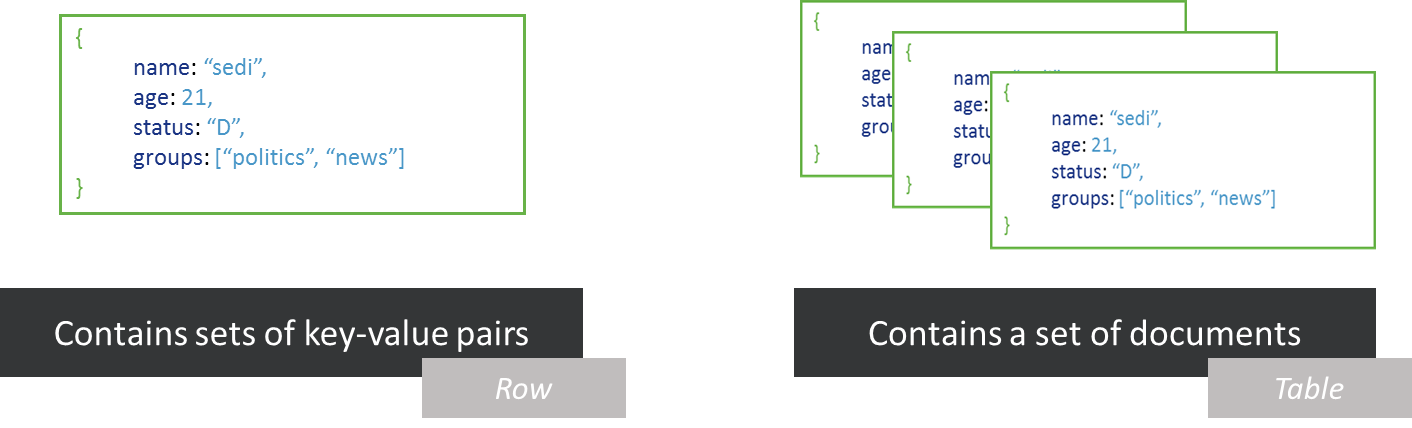
\includegraphics[width=\linewidth,keepaspectratio]{images/documentscollections.png}
\caption{Documents and collections}
\end{figure}
\\
MongoDB stores data as Binary JSON documents also known as BSON. The documents can have different schemas, which means that the schema can change dynamically as the application evolves. Automatic sharding enables data in a collection to be distributed across multiple systems for horizontal scalability as data volumes increase\cite{Edward2015}. Additional, MongoDB doesn’t only support Key-Value operations. It allows complex queries, aggregations and secondary indexes that unlock the value in structured, semi-structured and unstructured data. One of MongoDB’s major features is the support for many types of queries like text search, range queries, geospatial queries over to MapReduce queries\cite{MongoDBInc.2013a}.
\\
MongoDB was created by Dwight Merriman and Eliot Horowitz, who had encountered development and scalability issues with traditional relational database approaches while building Web applications at DoubleClick, an Internet advertising company that is now owned by Google Inc. The database was released to open source in 2009 and is available under the terms of the Free Software Foundation's GNU AGPL Version 3.0 commercial license. However, the database is one of the most popular NoSQL databases and is used by several company like Bosch, Facebook, Expedia and so on\cite{Hows2013}.

\section{Use Cases: What is MongoDB for?}
This section will give you an insight between the features and potential of MongoDB and some problems that is suited to solve.
\\
Beginning with online and mobile Apps. Nowadays Companies want their business on their smartphones or access it from everywhere through the web. In comparison to RDMBS MongoDB addresses the upcoming challenges of these plans. Furthermore, MongoDB promises to make it easier than other alternatives. Requirements for going mobile or online are hard to manage. For example, different types of device like smartphone or wearables are creating new types of unstructured and semi-structured data. Another reason is the number of devices and users. Meanwhile, Response times must keep and provide the same User experience. So, Scalability has now a high priority. MongoDB tries to decrease the degree of difficulty for these Requirements. That is why MongoDB offers a flexible data model and rich query functionality. Therefore, MongoDB can manage any kind of data, no matter how dynamically the data changes. In addition to that, MongoDB’s development concentrates on scalability and can handle a lot of Users and data sets\cite{MongoDBInc.2013a}.
\\
Another Example for a suited use case is a catalog. Mention that almost anybody knows some requirements a Catalog must meet. Deleting, creating and changing items or their features or their attributes – only to mention few - are a standard set of Requirement of a catalog. Behind the scenes, we see a lot of challenges for a RDMS. There will be a lot of changes in the data, like new data and new metadata to your catalogs. We already talked about the untrusted and semi-structured in the first Use case. Again, we got the same problems with a RDBMS. How does MongoDB make it easier for developers? First, it is how the data is structured in MongoDB. With MongoDB’s JSON document model makes it easy to store different assets with different attributes in a single place. It also makes it simple to represent complex, hierarchical relationships. Schemas in MongoDB are self-describing. You can add new products and features and evolve the schema instantly, without taking the database down or impacting performance. Lastly an expressive query language, indexing, including text search and geospatial, and analytics provide flexible access to the data, no matter how the application, business or developer needs to find it\cite{MongoDBInc.2013a}.
\\
All in all, these are only few examples for use cases and for what MongoDB is. In general MongoDB claims to be suited for high flexible data schemas to provide the ability for data changes, structed, unstructured and semi structured data. Additionally, MongoDB eco system let developer spend less time for the design of models, entities, relationships and tables, and more time on the application\cite{MongoDBInc.2013a}.

\section{Datamodel}
Before designing a database, it is crucial to analyse the data and the requirements of the application. In contrast to relational databases there is no strongly recommended way to structure your data, like for example a normalized data model to avoid inconsistencies on updates. However, there are well established patterns which help developers to create their data model \cite{Banker2016}. Later in this chapter, there will bw some examples for common design patterns. But at first, the following paragraphs will concentrate on the data concepts of MongoDB in detail.

\subsection{Databases and Collections}
As mentioned in the introduction, MongoDB is structured in databases collections and documents. MongoDB provides a mongo shell to communicate with the database. The code snippets provided in this chaptered can be performed on the mongo shell \cite{mdbdocu}.

A Database can hold collections of documents. The creation of a database occurs automatically when the first document is pushed to a collection of this database. Thus, there is no command to create an empty database \cite{mdbdocu}. The following commands show how simply it is to select and create a new database by inserting its first document.

\begin{lstlisting}[frame=single, caption=Create Database, label=createdb]
use newDatabase
db.newCollection.insertOne( { value: 2 } )
\end{lstlisting}


This example also shows the process of creating a new collection. As the database, the collection is created as soon as the first document got inserted. Certainly, there is also a function to explicitly create a new collection with an option to pass parameters affecting the collections behaviour. In the example in Listing \ref{createcol}, a collection with limited number of documents is created. All options can be found in the MongoDB documentation \cite{mdbdocu}.

\begin{lstlisting}[frame=single, caption=Create Collection, label=createcol]
db.createCollection( 'newCollection', { max: 1000 } )
\end{lstlisting}

\subsection{Documents}
MongoDB stores documents in the BSON format. This format supports multiple datatypes. Many of them are common in the information technology, such as Double, String or Boolean. A full list would go beyond the scope of this book, but can be found in the BSON specification. In general, there are all types needed for object oriented programming \cite{bsonspec}. The chapter Queries and CRUD operations will treat the way BSON types can be used to query through documents. But before that, the concept of documents will be explained.

\subsection{Embedded Documents and Referencing}
The below example in Listing \ref{embdoc} shows how a document is structured. The field name \_id is reserved to be used as primary key. It has some special characteristics like being unique in the collection and immutable. To make sure this field is unique, it is recommended to use a unique ObjectId. If there is no value submitted with the document, an ObjectId is generated automatically \cite{mdbdocu}. 

\begin{lstlisting}[frame=single, caption=Embedded Documents, label=embdoc]
var newDocument = {
	_id: <ObjectId>,
	birthdate: new Date('Jan 01, 1990'), 
	name: { 
        last:	 'Doe', 
        first: 'John' 
    },
	contact: {
		phone: '12345678',
		email: 'john@doe.com'
	}
}
\end{lstlisting}

Other fields can be added as needed. For example, a field containing the date of a person. Or an object containing the first and last name and another object with contact details. This concept of containing objects inside a document is called embedded sub-documents and has its own strength and weaknesses \cite{mdbdocu}. It may be resulting in a performance growth if the application always needs the document with its whole embedded data. But one common pattern for MongoDB says to consider whether embedded data or referencing is more suitable for the given situation \cite{Banker2016}. By referencing, the embedded data is stored in a separate document with a reference to its related document. This concept is the foundation for creating normalised data models. How this can be implemented for the document with John Doe can be seen in the code snippet in Listing \ref{refdoc}.

\begin{lstlisting}[frame=single, caption=Referencing Documents, label=refdoc]
var newPerson = {
	_id: <ObjectId1>,
	birthdate: new Date('Jan 01, 1990'), 
}

var newName = {
	_id: <ObjectId2>,
	user_id: <ObjectId1>,	
    last:	'Doe', 
    first: 'John'
}

var newContact = {
    _id: <ObjectId3>,
    user_id: <ObjectId1>,	
    phone: '12345678',
	email: 'john@doe.com'

}
\end{lstlisting}

When deciding whether referencing is reasonable, the atomicity of write operations also influences this decision. In MongoDB atomicity is only guaranteed on document level. As no single write operation can affect more documents, a normalised data model cannot be updated with one atomic operation. At this point denormalised data models have benefits over normalised ones. However, another design pattern for MongoDB is to overthink your overall database selection if you need atomic, consistent, isolated and durable operations, also known as ACID principles \cite{Banker2016}. 

\subsection{Validation}
MongoDB comes with a way to validate documents by itself. There are different ways to handle documents which do not match its validation criteria. By default, invalid documents are rejected with an error. A collection, which would check if the new document contains a birthdate, would look like the following in Listing \ref{valcol}. Furthermore, it is also possible the check the fields for a certain data type \cite{mdbdocu}.

\begin{lstlisting}[frame=single, caption=Validation for Collections, label=valcol]
db.createCollection( 'users', {
	validator: { 
	    $or: [ { 
	        birthdate: { $exists: true } 
	    } 
        ] 
    }
}
\end{lstlisting}
		
\section{Queries and CRUD operations}
MongoDB has several queries and operations to manage its data. This chapter gives a short overview of the most important operations.

\subsection{Create (Insert)}
Before searching for or working with data, the database needs information that can be worked with. How documents can be created was introduced while treating how to create a new database. This command inserts one document into a collection and can be found again in the Listing \ref{insdoc}. But there are also commands to insert an array of documents at once \cite{mdbbasics}.

\begin{lstlisting}[frame=single, caption=Create (Insert), label=insdoc]
db.newCollection.insertOne( {name: 'John', age: 30} )
db.newCollection.insertMany( [ 
    {name: 'Max', age: 20},
    {name: 'Marie', age: 25} 
] )
\end{lstlisting}

\subsection{Read (Find)}
To find data stored in a MongoDB, operations to either find one or multiple documents can be used. This example in Listing \ref{findoc} shows both operations. The difference is that the second operations stops after the first result and it is generally advised if only one result is excepted. Of course, the results can also be filtered by field values as shown in line three, or sorted by values as shown in line four \cite{mdbbasics}.

\begin{lstlisting}[frame=single, caption=Read (Find), label=findoc]
db.newCollection.find()
db.newCollection.findOne()
db.newCollection.find( { 'name.last': 'Doe' } )
db.newCollection.find().sort( { 'name.first': 1 } )
\end{lstlisting}

\subsection{Update}
MongoDB also provides a function to update documents with three input parameters: the search criteria, the new object and options. It is important to understand that any fields that are not part of the new object are also removed from the old object, as it were completely rewritten. The option upsert implies to add any fields that do not exist yet. It is also possible to update multiple options that match the search criteria with one command \cite{Banker2016}. An example for a basic update operation can be found in Listing \ref{upddoc}.

\begin{lstlisting}[frame=single, caption=Update, label=upddoc]
db.newCollection.update(
    { name: 'John' }, 
    { age: 21, name: 'John', lastname: 'Doe'  }, 
    { upsert: true } )
\end{lstlisting}

\subsection{Delete}

The last operation of CRUD examines the deletion of documents, collections or whole databases. The remove operation, as shown in line one of the code snippet in Listing \ref{deldoc}, removes all documents which match the criteria. The \_id field can help to be sure to only delete the right document. It can lead to conflicts if a documents is deleted without considering its references, because references from other documents will not change automatically \cite{mdbbasics}. Line 2 shows how to delete a collection and line 3 shows how to delete an entire database.

\begin{lstlisting}[frame=single, caption=Delete, label=deldoc]
db.newCollection.remove( { age: 20 } )
db.newCollection.drop()
db.dropDatabase()
\end{lstlisting}

\newcommand{\anfu}[1]{\glqq #1\grqq}
\newcommand{\anfuc}[2]{\anfu{#1}\cite{#2}}

\chapter{Architecture}
\section{Core Processes}
The MongoDB server package comes up with three main processes:
\begin{itemize}
  \item mongod
  \item mongo
  \item mongos
\end{itemize}
\textit{mongod} is the core database server. Once started, the \textit{mongod} listens by default on port 27017 for requests. It also manages the data format and performs all background operations. For administration the \textit{mondod} provides an HTTP interface witch can be reached at the localhost on port 28017 (1000 higher than the default port). The data directory \textit{mongod} connects to is by default C:\textbackslash data\textbackslash db (or /data/db). This directory definitely has to exist and the default ports have to be free, otherwise the process fails to start \cite{pracmong}.\\
The \textit{mongo} process is an interactive MongoDB shell. It gives the user the possibility to communicate with a running \textit{mongod} process via a JavaScript like query language. If running on the same host it automatically connects to the \textit{mongod} process and a preinstalled test database \cite{pracmong}.\\
The \textit{mongos} process is working like a routing service and is the basis for MongoDBs sharding ability that will be described later. It holds the information about where the requested data is located and forwards the request from an application server to the right destination \cite{pracmong}. \\
By running a \textit{mongod} process you already have a standalone deployment of MonogDB that can be accessed by a client. But in case of failure there is no redundancy or recovery, that prevents data loss, so its not recommended to use this in a production environment. To avoid this replication is used to guard against hardware failure or database corruption. It also gives the possibility to perform normally high-impact maintenance with little or no impact \cite{theguide}.

\section{Replication}
\anfuc{MongoDB supports the replication of a database’s contents to another server in real time or near real time}{theguide}. For that MongoDB provides two different replication methods. The traditional \textit{Master/Slave Replication} and \textit{Replication Sets}.

\subsection{Master/Slave Replication}
In a Master/Slave set up one \textit{mongod instance} acts as a master the others declared as slaves. All write and read operations are requested to the master and the slaves replicate the data of the master, but can't be requested by a client. If a failure occurs that forces the master to go down, the hole system can't be reached anymore. The data, till the last replication to the slaves, is saved, but can't be accessed until the master comes up again. \\
In MongoDB the master holds a capped collection called \textit{oplog}. The \textit{oplog} is an ordered history of all logical writes that are executed within a defined time period. The operations stored in the \textit{oplog} in an idempotent way, so they can be performed multiple times without changing the result \cite{pracmong}. That's useful when a slave runs into failure while executing the operations onto its data. In that case the replication process can be simply restarted. If the slaves syncing process last to long or the slave was down for a longer time, the oplog data could be deleted before the slave was able to synchronize \cite{pracmong}. In that case the slave has to start a resync process. To avoid such a situation the oplog length should be chosen in consideration of the slaves performance.\\
The configuration of MongoDB with a \textit{Master/Slave Replication} is only recommended for more than 50 nodes \cite{pracmong}. At that point the next described replication method the \textit{Replica Set} is reaching its limits, because the communication overhead becomes to big.

\subsection{Replica sets}
In contrast to the \textit{Master/Slave Replication} in a \textit{Replica Set} no fixed master is defined. Instead the nodes are declared as primary or secondary. Each node in a \textit{Replica Set} can become primary, but there is only one primary at a time, the others are secondaries. All write operations going through the primary, but read operations can also be performed by secondaries \cite{pracmong}. The replication process works just like it does in a \textit{Master/Salve Replaction}, but if a primary goes down a new primary is elected out of the secondaries.

\subsubsection{Communication}
All nodes in a \textit{Replica Set} communicate with each other. As life sign they are sending a heartbeat signal to each node and getting back status replies of each node. Those replies contain information about the node, such as is he primary or secondary and what type of node he is. Each node can be assigned a certain number of votes and a priority.\\
This results in a various types of nodes:
\begin{itemize}
  \item \textbf{normal secondaries:} hold a copy of the primaries data, accept read requests and are primary candidates
  \item \textbf{priority-0-members:} secondaries that will never become primary
  \item \textbf{hidden-members:} priority-0-members that can't serve read request, because they are hidden for the client
  \item \textbf{delayed-members:} have a delay in synchronization to prevent human failure
  \item \textbf{arbiters:} don't hold data, they just solve ties in a election process
  \item \textbf{non-voting-members:} normal secondaries, but they can't vote
\end{itemize}
If the primary recognizes that the heartbeat of a secondary has stopped he has to check if he still can reach the majority of the set and if it can't he demotes itself to secondary and starts a election process. Also the election process is started if a secondary recognizes the primary is down. All voting nodes now collect the for the election required information form the primary candidates. The election of a primary depends on various parameters. Important is that the elected node has the most recent data of all nodes. The candidate with the most votes is promoted to primary. When the old primary comes up again he will be a new secondary \cite{pracmong,theguide}.

\subsubsection{Consitency}
The replication in MongoDB works asynchronously. Writes are always routed to the primary, but reads can also requested to a secondary. \anfuc{This behavior is characterized as eventual consistency, witch means that although the secondary's state is not consistent with the primary node state, it will become consistent over time}{pracmong}. It is possible to configure the preferred reading node by primary, primaryPrefferd, secondary, secondaryPreffered or nearest \cite{theguide}. The only way to ensure that a client always requests the up to date data is to set the read preference to primary. But in this situation we only get the traditional \textit{Master/Slave} behaviour and we loose all availability features. Normally the read preference would be set to primaryPreffered, so reads were just send to the secondaries if the primary is unavailable. Or if the system is widely distributed nearest would be chosen.
To ensure a minimum number of secondaries is up to date it is possible to specify write concerns. With write concerns the client will get the success response only after the write operation was replicated to the specified number of secondaries \cite{pracmong}.

\section{Sharding}
If the amount of data exceeds the capacity of a single database server, partitioning is needed to distribute the data on multiple servers. For MongoDB this ability is even more important, because it uses memory mapped file I/O to access its underlining data storage\cite{theguide}. For that MongoDB uses a horizontal partitioning mechanism called \textit{sharding}.\\
The data collection gets divided and distributed onto multiple servers called shards. Every shard is an independent database managed by a \textit{mongod} process. All the shards are combined to one logical database. The partitioning and routing are managed by the earlier mentioned \textit{mongos} process. All write and read requests of an application are send to a \textit{mongos} process, that holds the information where the requested data is stored and forwards the request to responsible \textit{mongod} process. Also the partitioning decision is taken by the \textit{mongos} process. The data is distributed based on a configured shard key and chunk size. The metadata of a sharded cluster is stored on special config servers, where the \textit{mongos} processes can obtain the routing information.

\section{Summary}
Figure \ref{arch-example} describes one possible deployment architecture that contains all in this chapter mentioned artifacts. Clients can connect to a \textit{mongos} process running on an application server. This process forwards the requests based on the information stored on the \textit{config servers} to the right shard. A shard is an replica set containing several \textit{mongod} processes.
\begin{figure}[H]
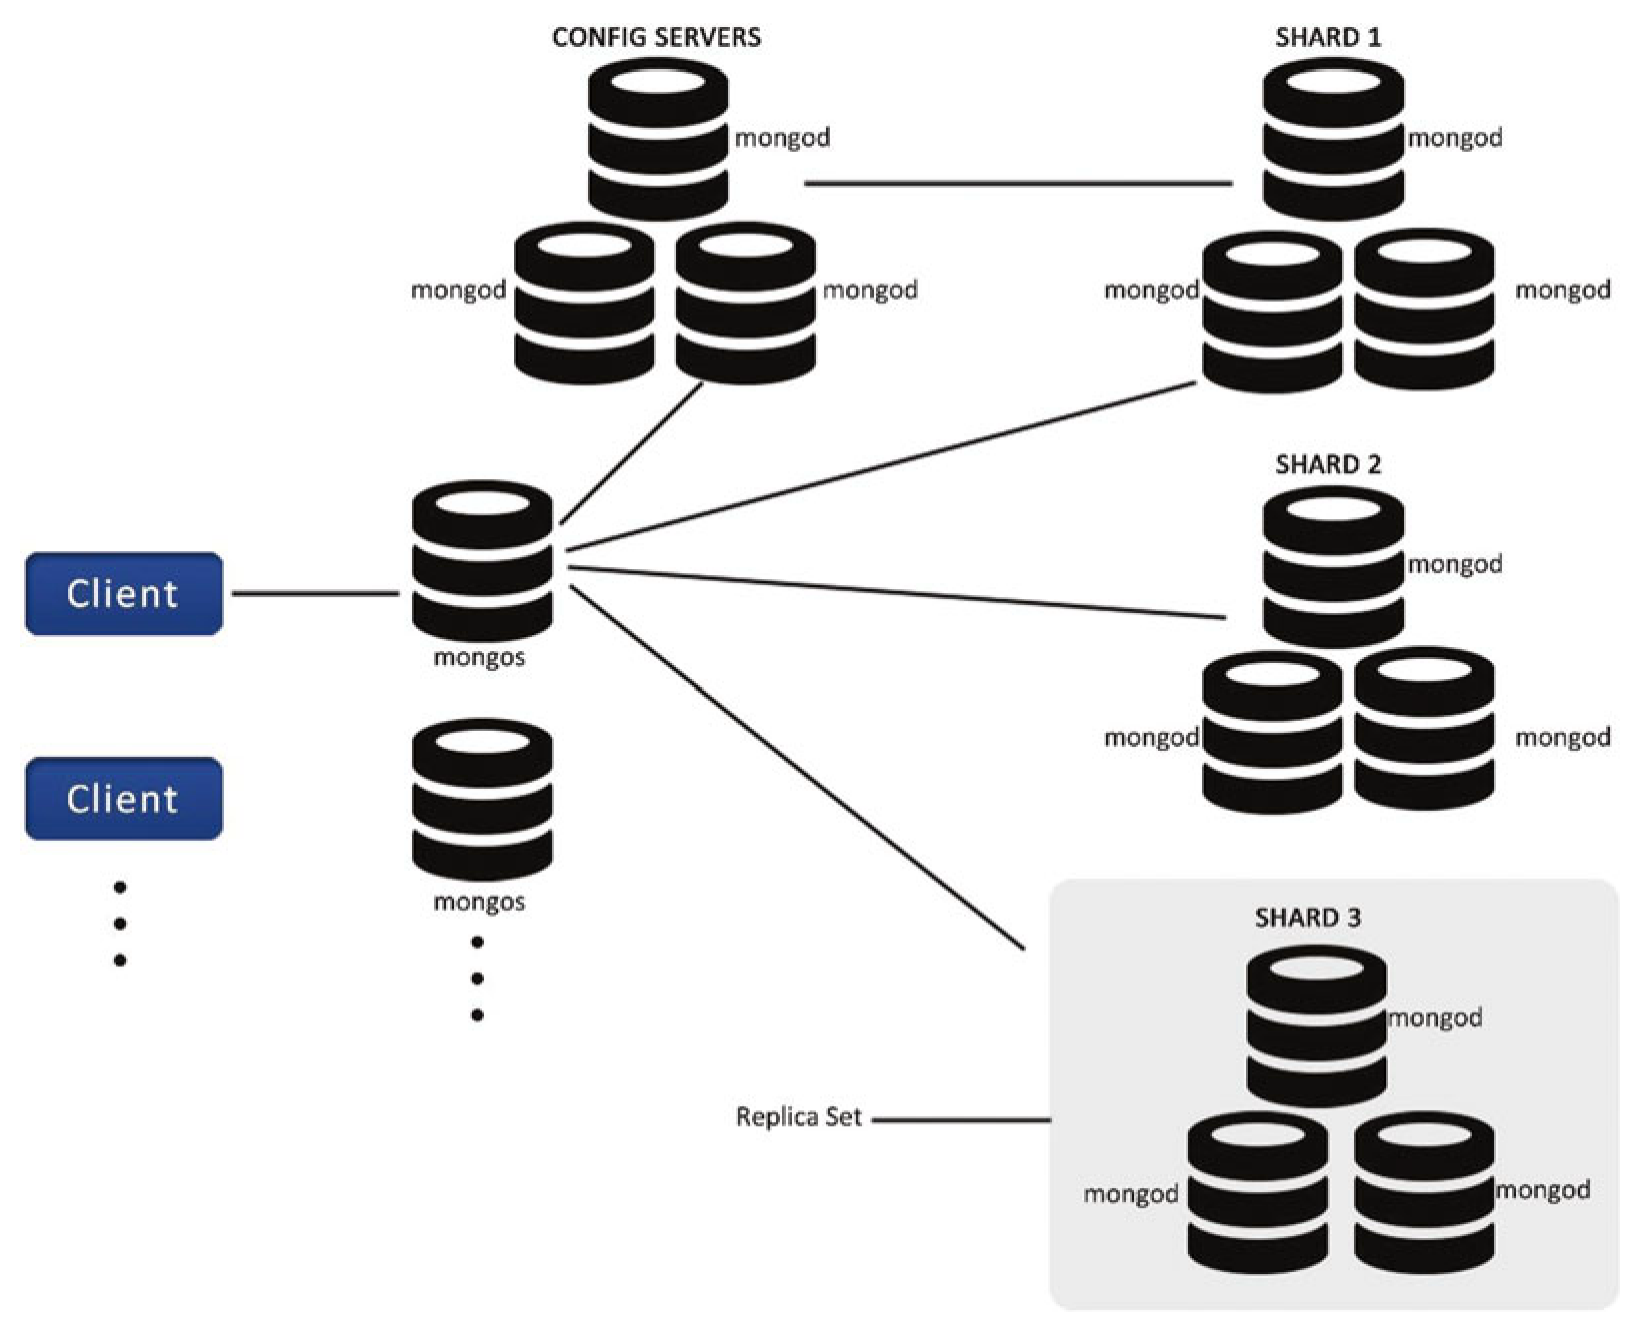
\includegraphics[width=\linewidth,keepaspectratio]{images/deployment.png}
\caption{MongoDB Architecture Example}
\label{arch-example}
\end{figure}



\section{Performance}
\subsection{Performance measurement introduction}
Before a performance measurement or comparison between database systems can be made, it is necessary to define the performance indicators. Depending on the use-case of the measured databases the results can be completely different. For example a real-time system is a lot more dependent on access times, latency and fast updates for concurrent users. A scientific database has to be fast at processing complex queries with joints and preprocessing routines like aggregation \cite{Neil_O}. Of course the benchmark should be implemented to test the performance of a database system in a way that reflects your usage in the future.
\\\\
For database systems there is a council called the TPC . This organization tests different database systems on physical and virtual machines and scores them by performance. The performance indicators can be seen on their website and there are different benchmarks depending on the use-case of the system \cite{_tpc.org.}. 
\\\\
Another standardized benchmark for database implementations is the Wisconsin Benchmark. This was one of the first standardized benchmarks and was made for relational databases. The test contains of inserts, selections, joints and projections. For further details on this benchmark, see the paper \cite{DeWitt_The_1991}.
\\\\
This paper will summarize MonogDB performance compared to other popular NoSQL and SQL  databases.

\subsection{Influencing factors to database performance}
All the results provided by this paper are dependent on the underlying hardware used. Depending on the host system for the database application, the performance can vary a lot \cite{Lee_W._2009}. Examples for big performance factors are available memory, processor speed and the used storage.
\\\\
For evaluation which database system should be used, it is important to know on what kind of hardware the production system will run. This is due to the fact, that different database systems were developed to meet certain performance goals on different hardware. Therefore some databases scale well with more memory and memory bandwidth since they try to cache a lot of the data in system memory. But there are also databases which try to be very lightweight on memory for low end systems or massive I/O  operations \cite{Boncz_Database_1999}.
\\\\
Nearly all databases are reliant on the used storage. This storage is the only way to keep the data, even when the system is turned off. Even In-memory databases use the persistent storage to save their current data \cite{Wang_Main_2001}. As transactions ultimately have to be written to the storage, this becomes the biggest bottleneck. With traditional HDDs having a high latency when accessing random data, which happens frequently on a database system, the introduction of SSDs  eliminated those problems. Benchmarks done on traditional HDD storage can be translated most of the time to SSDs since all databases will perform better but should stay at the same relative performance.
\subsection{NOSQL compared to SQL databases}
It is often one of the first question, when talking about database performance. SQL or NOSQL, which one is faster? Comparing those two types of databases generally, is not really useful. The way how data is stored is completely different and the use-case defines if SQL or NOSQL fits better.
\\\\
A good example for the difference of these two types is Twitter. They use a NOSQL database for all the tweets. Although Twitter is using MySQL heavily. The reason for this is easy to explain. A tweet contains some sort of content like text or images and a lot of additional information like hashtags, user and topics. Storing that data in a relational, normalized way, it would take a lot of tables and joins to represent a tweet . All hashtags would be referenced over multiple tables. These joins take time and since Twitter is a real time platform, latency should be low \cite{Weil_21}.
\\\\
In contrast the NOSQL implementation is way easier. The complete Tweet is stored as a document. The hashtags and links are stored in the same document in a key value manner. Now when you want to read 100 Tweets, in a NOSQL context, this can be done by one simple query. In a relational model, complex joins for each Tweet would be necessary. In such a scenario performance is obviously on the NOSQL side, but only because the use-case is well suited for non-relational models.
\subsection{MongoDB performance}
This paper will be limited to benchmarks of low level functions for databases. These functions are: reads, writes and deletions. Performance is measured between MongoDB and MariaDB. MariaDB is a SQL database and as previously mentioned, general comparisons between NOSQL and SQL are not useful. In this case two implementations of SQL and NOSQL are compared which is relevant when the use-case can be implemented by both designs without drawbacks. In such a scenario, raw performance is a valid factor.
In addition to the benchmark implemented by the author of this section, another one is used for validity and a broader overview. The referenced paper contains additional databases.
\\\\
The following performance test were performed, using NodeJS. For MongoDB connectivity the official MongoDB driver  was used. The same applies for the MariaDB driver . The driver selection can cause huge performance differences. There are several MariaDB drivers for NodeJS and of course other programming languages. Therefore comparisons of database performance should be done, using the same programming language \cite{_mscdex.}. The inserted data contains just an id represented by an integer.
\begin{figure}[H]
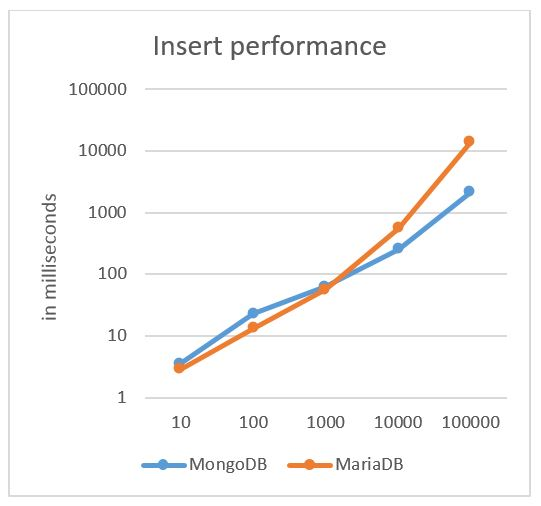
\includegraphics[width=\linewidth,keepaspectratio]{images/Performance_Inserts.JPG}
\caption{Insert MongoDB vs MariaDB}
\label{arch-example}
\end{figure}
\begin{figure}[H]
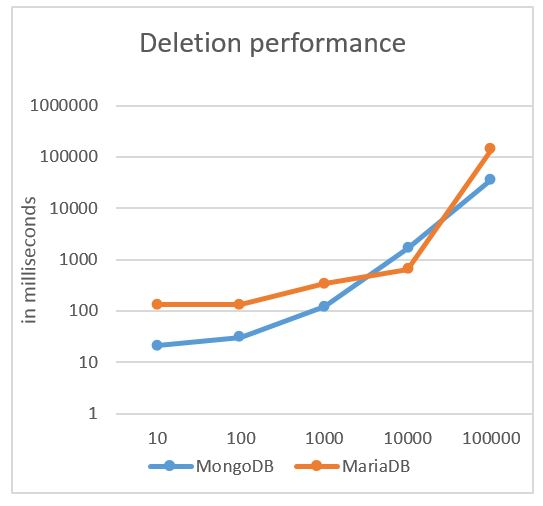
\includegraphics[width=\linewidth,keepaspectratio]{images/Performance_Deletion.JPG}
\caption{Deletion performance}
\label{arch-example4}
\end{figure}

The numbers show an interesting result. In the insert test MongoDB performs worse than MariaDB just slightly up to the point of 1000 inserts. After that point MariaDB falls behind. With increasing number of inserts the performance leap of MongoDB increases a lot. A reason for this could be some kind of overhead for inserts on MongoDB, further investigation is needed to evaluate the results and the cause. A similar behavior can be seen on deletion test.
\\\\
The following performance results are provided by the paper \cite{Li_A_2013}
\begin{figure}[H]
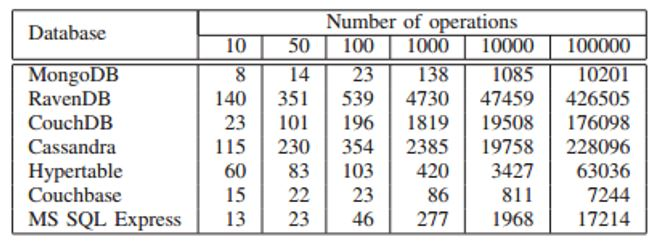
\includegraphics[width=\linewidth,keepaspectratio]{images/Performance_Reads.JPG}
\caption{time for read operations in milliseconds}
\label{arch-example2}
\end{figure}
\begin{figure}[H]
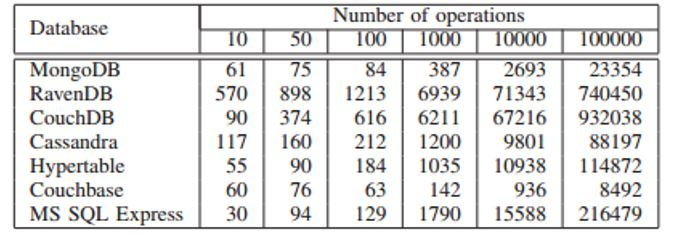
\includegraphics[width=\linewidth,keepaspectratio]{images/Performance_Writes.JPG}
\caption{time for write operation in milliseconds}
\label{arch-example3}
\end{figure}
\begin{figure}[H]
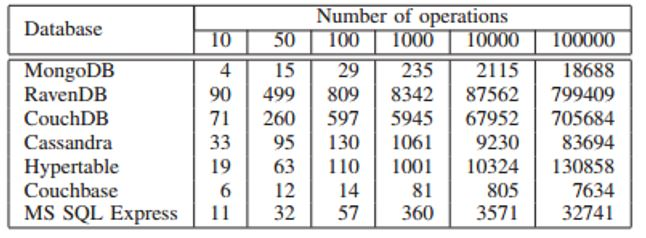
\includegraphics[width=\linewidth,keepaspectratio]{images/Performance_Delete.JPG}
\caption{time for delete operation in milliseconds}
\label{arch-exampl1}
\end{figure}

Interestingly the benchmarks from the paper show similar results on write performance when comparing the SQL implementation and MongoDB. After 100 writes MongoDB performs better. When comparing to other NoSQL databases, MongoDB is always in the upper half of the field. So it can be said, that this database should be suited well for demanding applications and performance shouldn't be a major problem. 
\\\\
These statements only apply for single instance usage. Since MongoDB uses a single master architecture for multiple instances, throughput will be less than database systems that trade consistency for performance. Using sharded servers can increase performance for horizontal scaling. With this addition, MonngoDB is also very usable for scientific applications with high amounts of I/O and data \cite{Dede_Performance_2013}.




\section{MongoDB and Big Data}
In terms of Mobile Applications, IoT, Industry 4.0 and cloud-computing, data is vast, unstructured, sometimes unwieldy and complicated. In this context, Big Data is identified by its velocity, variety and volume. Therefore, requirement and expectations has changed how to store, process and analyze data. It has led to the development of NoSQL databases such as MongoDB\cite{MongoDBInc.2013}.
\\
However, in the era of Big Data, there a 2 kind of database solutions for facing Big Data. We distinguish operational Big Data Systems and analytical Big Data solutions. Features of Operational Big Data Systems provides real-time, interactive, dynamic workloads that ingest and store data. MongoDB belongs to this category and is a popular technology for operational Big Data applications\cite{MongoDBInc.2013}.
\\
On the other hand, Analytical Big Data technologies are useful for retrospective, sophisticated analytics of your data. A most-known example of an Analytical Big Data technology is Apache Hadoop. Hadoop is designed for storing and processing large sets of data on a distributed environment based on commodity servers and storage. It is an open-source Apache project, which consists of a distributed file system called HDFS (Hadoop Distributed File System) and a data processing and execution model called MapReduce\cite{Wadkar2014}.
\\
Choosing between operational and analytical Big Data solution isn’t the right way of thinking about facing this Decision. Many organizations are harnessing the power of Hadoop and MongoDB together to create complete big data applications. At the one hand, MongoDB powers the online, real time operational application, serving business processes and end-users, exposing analytics models created by Hadoop to operational processes. At the other hand, Hadoop consumes data from MongoDB, blending it with data from other sources to generate sophisticated analytics and machine learning models. Results are loaded back to MongoDB to serve smarter and contextually-aware operational processes – i.e., delivering more relevant offers, faster identification of fraud, better prediction of failure rates from manufacturing processes\cite{MongoDBInc.2013}.
\\
In the following, you see a Figure which shows a Design pattern how to combine these two technologies to be ready for a Big Data environment:
\begin{figure}[H]
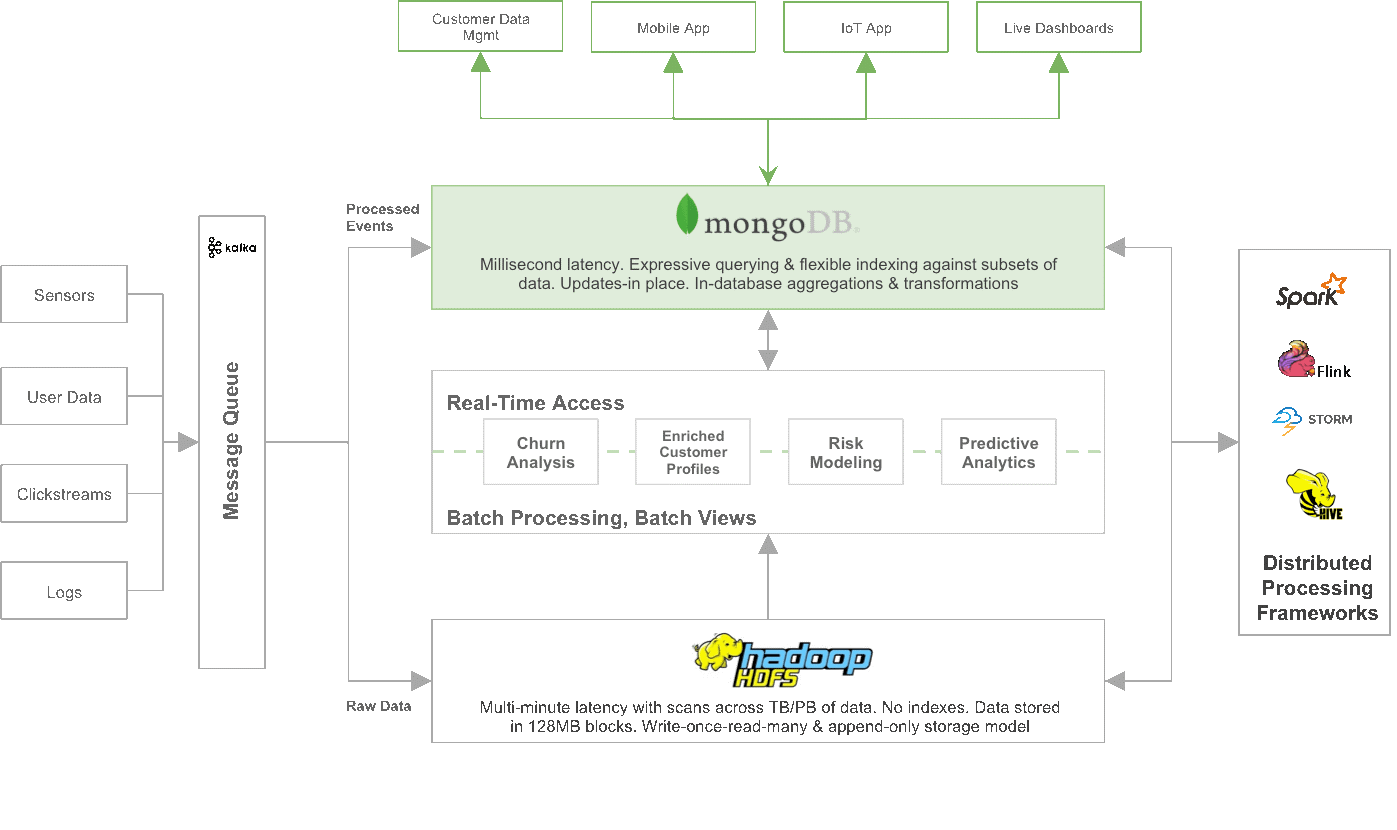
\includegraphics[width=\linewidth,keepaspectratio]{images/bigdata.png}
\caption{Design pattern for integrating MongoDB with Data Lake~\protect\cite{MongoDB2016}}
\end{figure}

\section{Conclusion}
All in all, MongoDB is a powerful and popular documented-oriented database. It comes with a lot of features, which meets the modern-day requirements and challenges for business applications, platforms and the web. 
The examples about the MongoDB data model, queries and CRUD operations showed how easy it is for developers to setup and work with this database. MongoDB is also very flexible in terms of extending the structure of documents. However, it is strongly recommended to consider the usage of common patterns to create a strong and future-proof data model. The usage of patterns will also help developers to understand a given database structure and work together on larger projects.
Even in a big data context MongoDB is a good choice for big data applications. That is why you will find a lot of companies and startups using MongoDB in their development.

\subsection{MongoDB in CAP-Theorem}
In a single server or Master/Slave configuration MongoDB prioritize consistency over availability. That might be the reason why in most literature MongoDB is positioned at CP-side of the CAP-Theorem. But in \textit{Replica Sets} it is possible to trade some of the consistency for a higher availability, by configuring \textit{read preferences} (\ref{read-write}). By allow reading from secondaries, there is no way to ensure the client is reading consistent data. \anfuc{This behavior is characterized as eventual consistency, witch means that although the secondary's state is not consistent with the primary node state, it will become consistent over time}{p. 108}{Edward2015}. With \textit{write concerns} (\ref{read-write}) it is possible to obviate inconsistent reads happen to often, by ensure that a minimum number of secondaries is consistent. \\
Figure \ref{mongodb-cap} describes how the three values change depending on the configuration. The partition tolerance is always fulfilled, because MongoDBs architecture is designed that way. By allow reading from secondaries availability will be increased at the expense of consistency and some consistency can be recovered using \textit{write concerns}. But availability is always limited to reading, so it can never be fulfilled for all aspects of an application.
\begin{figure}[H]
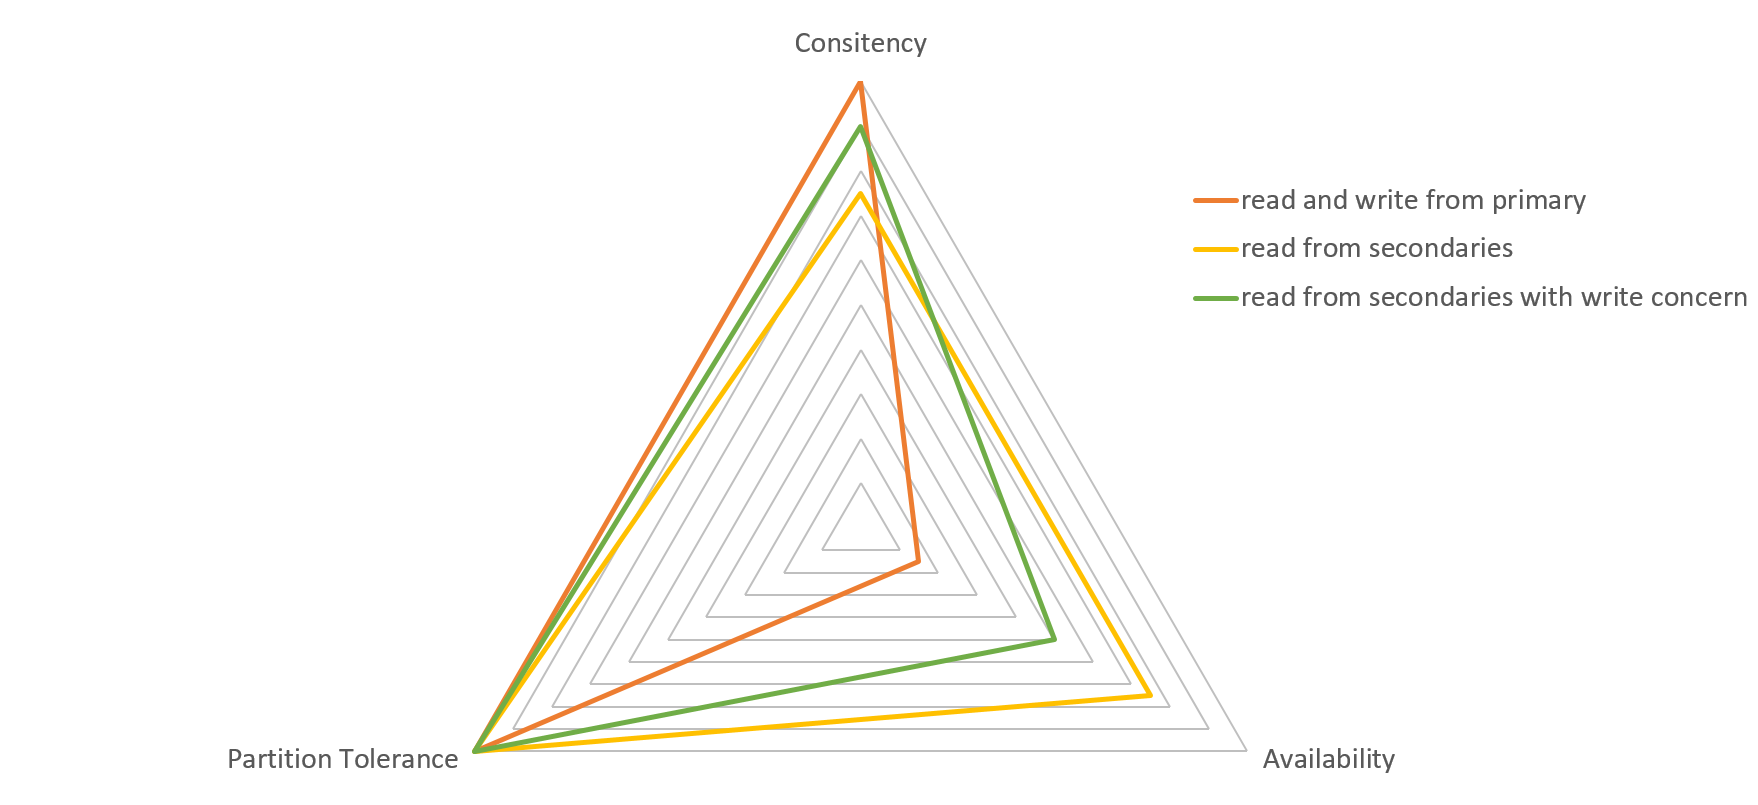
\includegraphics[width=\linewidth,keepaspectratio]{images/mongodb-cap.png}
\caption{Write process with write concerns}
\label{mongodb-cap}
\end{figure}
	
	\clearpage
		
	\pagenumbering{roman}
	
	% Literaturverzeichnis
	\cleardoublepage
% 	\printbibheading
% 	\printbibliography[nottype=online,heading=subbibliography,title={Publikationen}]
% 	\printbibliography[type=online,notkeyword=Gesetz,notkeyword=Standard,heading=subbibliography,title={Online Quellen}]
% 	\printbibliography[type=online,keyword=Gesetz,heading=subbibliography,title={Rechtsquellenverzeichnis}]
% 	\printbibliography[type=online,keyword=Standard,heading=subbibliography,title={Standards \& Normen}]
% 
% 	\renewcommand\bibname{Literaturverzeichnis}
% 	\printbibliography
  \bibliographystyle{apacite}
  \bibliography{bibliographie}
	%\newpage\null\thispagestyle{plain}\newpage
	%\newpage
	% Glossar
	%\printglossary[style=altlist,title=\langglossar]
	%%!TEX root = ../dokumentation.tex

%
% vorher in Konsole folgendes aufrufen:
%	makeglossaries makeglossaries dokumentation.acn && makeglossaries dokumentation.glo
%

%
% Glossareintraege --> referenz, name, beschreibung
% Aufruf mit \gls{...}
%
\newglossaryentry{Glossareintrag}{name={Glossareintrag},plural={Glossareinträge},description={Ein Glossar beschreibt verschiedenste Dinge in kurzen Worten}}

\newglossaryentry{Commodity-Hardware}{name={Commodity-Hardware},description={\flqq Computer hardware that is affordable and easy to obtain. Typically it is a low-performance system that is IBM PC-compatible and is capable of running Microsoft Windows, Linux, or MS-DOS without requiring any special devices or equipment.\frqq\footcite{Beal.2015}}}

\newglossaryentry{Git}{name={Git},plural={Git},description={Git ist ein kostenloses System zur Versionskontrolle für kleine wie auch sehr große Projekte. ({\url{http://git-scm.com/}})}}

\newglossaryentry{NetBeans}{name={NetBeans},plural={NetBeans},description={The Smarter and Faster Way to Code Quickly and easily develop desktop, mobile and web applications with Java, HTML5, PHP, C/C++ and more. NetBeans IDE is FREE, open source, and has a worldwide community of users and developers. ({\url{https://netbeans.org}})}}

\newglossaryentry{Maven}{name={Maven},plural={Maven},description={Apache Maven is a software project management and comprehension tool. Based on the concept of a project object model (POM), Maven can manage a project’s build, reporting and documentation from a central piece of information. \\ ({\url{http://maven.apache.org/}})}}

\newglossaryentry{Nagios}{name={Nagios},plural={Nagios},description={Nagios Is The Industry Standard In IT Infrastructure Monitoring. Achieve instant awareness of IT infrastructure problems, so downtime doesn't adversely affect your business. Nagios offers complete monitoring and alerting for servers, switches, applications, and services. \\ ({\url{https://www.nagios.org}})}}

\newglossaryentry{Zabbix}{name={Zabbix},plural={Zabbix},description={Zabbix is the ultimate enterprise-level software designed for real-time monitoring of millions of metrics collected from tens of thousands of servers, virtual machines and network devices. Zabbix is Open Source and comes at no cost. \\ ({\url{http://www.zabbix.com}})}}

\newglossaryentry{Bootstrapping}{name={Bootstrapping},description={\flqq The computer term bootstrap began as a metaphor in the 1950s. In computers, pressing a bootstrap button caused a hardwired program to read a bootstrap program from an input unit. The computer would then execute the bootstrap program, which caused it to read more program instructions. It became a self-sustaining process that proceeded without external help from manually entered instructions. As a computing term, bootstrap has been used since at least 1953.\frqq\footcite[S. 1273]{Buchholz.1953}}}

\newglossaryentry{Generic}{name={Generic},plural={Generics},description={Ein Interface oder eine Klasse kann mit einem oder mehreren Parametern, den sog. Generics, definiert werden, welche zusätzliche Typangaben enthalten. Diese werden in spitzen Klammern notiert. Generics führen implizit einen Typumwandlung durch, welcher ohne Generics explizit erfolgen müsste\footcite[Vgl.][S. 4 f.]{Naftalin.2006}}}

\newglossaryentry{Plugin}{name={Plugin},plural={Plugins},description={\flqq Zusatzprogramm, welches über eine vordefinierte Schnittstelle in ein Basisprogramm eingebunden wird und dessen Funktionsumfang erweitert. [...] [Stammen] oftmals von anderen Herstellern als das Basisprogramm. [...] Plug-ins sind oft aus eigenständigen Programmen entstanden und können deshalb [...] i.d.R. auch ohne das Basisprogramm verwendet werden\frqq\footcite[]{Lackes.2015}}}
	

\end{document}
